% !TEX program = xelatex
\documentclass[11pt,a4paper]{article}

% ----------------------------------------------------------------------
% Academic Packages & Engine Configuration
% ----------------------------------------------------------------------
\usepackage{iftex}
\ifXeTeX
  \usepackage{fontspec}
  \IfFontExistsTF{Kalpurush}{
    \newfontfamily\bengalifont{Kalpurush}[Script=Bengali]
  }{
    \IfFontExistsTF{Noto Serif Bengali}{
      \newfontfamily\bengalifont{Noto Serif Bengali}[Script=Bengali]
    }{
      \IfFontExistsTF{Nirmala UI}{
        \newfontfamily\bengalifont{Nirmala UI}[Script=Bengali]
      }{
        \newfontfamily\bengalifont{FreeSerif}[Script=Bengali]
      }
    }
  }
  \newcommand{\bn}[1]{{\bengalifont #1}}
\else
  \usepackage[utf8]{inputenc}
  \usepackage[T1]{fontenc}
  \usepackage{lmodern}
  \newcommand{\bn}[1]{#1}
\fi

\usepackage{geometry}
\geometry{top=2.5cm, bottom=2.5cm, left=2.6cm, right=2.6cm}

\usepackage{setspace}
\setstretch{1.12}

\usepackage{amsmath,amssymb,amsfonts}
\usepackage{graphicx}
\usepackage{booktabs}
\usepackage{multirow}
\usepackage{tabularx}
\usepackage{array}
\usepackage{float}
\usepackage{cite}
\usepackage{xcolor}
\usepackage{tikz}
\usetikzlibrary{shapes.geometric, arrows.meta, positioning, calc, backgrounds, fit}
\usepackage{pgfplots}
\pgfplotsset{compat=1.18}
\usepackage{hyperref}
\hypersetup{
    colorlinks=true,
    linkcolor=blue!70!black,
    citecolor=blue!70!black,
    urlcolor=blue!70!black
}
\usepackage{caption}
\usepackage{subcaption}
\usepackage{enumitem}
\usepackage{algorithm}
\usepackage{algpseudocode}
\usepackage{titlesec}

% Section styling
\titleformat{\section}{\large\bfseries}{\thesection.}{0.5em}{}
\titleformat{\subsection}{\normalsize\bfseries}{\thesubsection.}{0.5em}{}
\titleformat{\subsubsection}{\small\bfseries}{\thesubsubsection.}{0.5em}{}

% ----------------------------------------------------------------------
% Document Metadata
% ----------------------------------------------------------------------
\title{\textbf{\LARGE Context Aware Bangla Text Analyzer for Sentiment, Sarcasm, and Hate Speech Detection}}

\author{
    \textbf{Md. Tariful Islam Jony}\textsuperscript{1} \qquad \textbf{Siyam Khan}\textsuperscript{2} \\[0.4em]
    \textsuperscript{1,2}Department of Computer Science and Engineering \\
    Khulna University of Engineering \& Technology (KUET), Khulna-9203, Bangladesh \\
    \texttt{\{2107119, 2107120\}@stud.kuet.ac.bd} \\[0.6em]
    \textit{Course: CSE 4122 (Natural Language Processing Laboratory)} \\
    \textit{Academic Term: 4th Year, 1st Term (CSE 4-1)}
}

\date{\vspace{-1.0em}}

% ----------------------------------------------------------------------
% Main Document Content
% ----------------------------------------------------------------------
\begin{document}

% ======================================================================
% Official KUET Project Report Cover Page
% ======================================================================
\begin{titlepage}
\centering

% KUET Official Logo
\vspace*{0.5cm}

\includegraphics[width=2.5cm]{figures/kuet_logo.png} \\[0.7cm]

% Institution Details
{\bfseries\large KHULNA UNIVERSITY OF ENGINEERING \& TECHNOLOGY} \\[0.3em]
{\normalsize Department of Computer Science and Engineering} \\[0.25em]
{\normalsize Khulna-9203, Bangladesh} \\[1.4cm]

% Course Title & Document Type
{\normalsize CSE 4122: Natural Language Processing Laboratory} \\[0.4em]
{\normalsize Project Report} \\[1.3cm]

% Project Title
{\bfseries\Large Context Aware Bangla Text Analyzer for}\\[0.4em]
{\bfseries\Large Sentiment, Sarcasm, and Hate Speech Detection}\\[1.8cm]

% Submitted By Section
{\bfseries\normalsize SUBMITTED BY} \\[0.8cm]
\begin{tabular*}{0.85\textwidth}{@{\extracolsep{\fill}}cc}
\textbf{Md. Tariful Islam Jony} & \textbf{Siyam Khan} \\[0.35em]
Roll: 2107119 & Roll: 2107120
\end{tabular*} \\[1.6cm]

% Submitted To Section
{\bfseries\normalsize SUBMITTED TO} \\[0.8cm]
\begin{tabular*}{0.95\textwidth}{@{\extracolsep{\fill}}cc}
\textbf{Dr. K. M. Azharul Hasan} & \textbf{Md Nazirulhasan Shawon} \\[0.35em]
Professor & Assistant Professor \\[0.35em]
Department of Computer Science and & Department of Computer Science and \\[0.2em]
Engineering, KUET & Engineering, KUET
\end{tabular*}

\vfill
\end{titlepage}

\clearpage
\pagenumbering{arabic}



\begin{abstract}
\noindent Understanding user-generated content in Bengali presents significant challenges due to informal spelling variations, colloquial expressions, and the widespread use of sarcasm. Standard natural language processing (NLP) pipelines typically treat sentiment analysis, sarcasm detection, and hate speech identification as isolated tasks. However, in online discourse, these dimensions are strongly interdependent. Sarcastic remarks frequently employ positive vocabulary to convey caustic negative critiques, which leads conventional classifiers to misjudge the true polarity. In this project, we develop a context aware multi-task text analysis system that evaluates all three dimensions across 218,371 annotated Bengali sentences (156,010 for sentiment polarity, 12,089 for sarcasm detection, and 50,272 for hate speech identification). We systematically implement and compare three progressive modeling paradigms: (1) a statistical machine learning baseline using sublinear TF-IDF with class-balanced Logistic Regression; (2) a deep sequential recurrent architecture using 128-dimensional dense word representations with a 2-layer stacked Bidirectional Long Short-Term Memory (BiLSTM) network; and (3) a pre-trained transformer architecture fine-tuning the 110-million parameter \texttt{BanglaBERT} model. Additionally, we implement a custom negation-preserving preprocessing pipeline that protects critical syntactic negation markers from destructive stopword filtering. Our empirical evaluation shows that fine-tuned \texttt{BanglaBERT} achieves strong performance across tasks, reaching 91.59\% accuracy and 91.58\% Macro F1 on hate speech detection, and 76.76\% accuracy and 74.89\% Macro F1 on sarcasm detection. Finally, we implement a context aware cross-task ensembling engine that resolves sarcastic polarity inversion and filters neutral factual statements.
\end{abstract}

\vspace{0.4em}
\noindent\textbf{\textit{Keywords:}} Bengali NLP, Sentiment Analysis, Sarcasm Detection, Hate Speech Detection, BanglaBERT, Bidirectional LSTM, Context Aware Classification, Empirical Benchmarking.

% ----------------------------------------------------------------------
\section{Introduction}
% ----------------------------------------------------------------------
Bengali is the seventh most spoken language in the world, with over 300 million native speakers primarily in Bangladesh and eastern India. Despite this large speaker population, computational tools for Bengali remain limited by challenges such as high morphological inflection, rich dialectal diversity, and a scarcity of standardized public benchmarks~\cite{alam2021banglabert}.

In online social platforms, comments and reviews often feature colloquial idioms, creative misspellings, and figurative language. Among these linguistic devices, sarcasm creates a substantial challenge for automated text understanding. Consider the following common type of social media review:
\begin{center}
\bn{“বাহ! কী অসাধারণ সার্ভিস, তিন ঘণ্টা অপেক্ষা করেও কোনো কাজ হলো না!”} \\
\small{(Translation: ``Wow! What extraordinary service, even after waiting three hours nothing was done!'')}
\end{center}

Under traditional bag-of-words or lexicon-based methods, positive words such as \bn{“অসাধারণ”} (\textit{oshadharon}, meaning extraordinary) heavily bias the classifier toward predicting positive sentiment. However, the subsequent clause \bn{“কাজ হলো না”} (\textit{kaj holo na}, meaning nothing was done) completely reverses the meaning into a negative assessment. A standalone sentiment analyzer lacks the context required to resolve this contradiction without input from a dedicated sarcasm detection component. At the same time, content moderation systems must distinguish between satirical remarks and harmful toxicity or cyberbullying.

\begin{figure}[htbp]
\centering
\resizebox{0.96\textwidth}{!}{%
\begin{tikzpicture}[
    node distance=1.0cm and 0.6cm,
    font=\sffamily\footnotesize,
    box/.style={draw=blue!80!black, fill=blue!5, rounded corners=4pt, thick, align=center, inner sep=6pt},
    data/.style={draw=green!60!black, fill=green!5, rounded corners=4pt, thick, align=center, inner sep=6pt},
    proc/.style={draw=orange!80!black, fill=orange!5, rounded corners=4pt, thick, align=center, inner sep=6pt},
    engine/.style={draw=red!80!black, fill=red!5, rounded corners=4pt, thick, align=center, inner sep=6pt},
    arrow/.style={-{Latex[length=2.2mm, width=1.4mm]}, thick, draw=gray!80!black}
]
    % Pipeline Nodes
    \node[data] (raw) {Multi-Task Corpora\\Sentiment ($N=156,010$)\\Sarcasm ($N=12,089$)\\Hate Speech ($N=50,272$)};
    \node[proc, right=0.8cm of raw] (prep) {Preprocessing\\Noise Filtering\\Zero-Width Removal\\Negation Protection};
    \node[box, right=0.8cm of prep] (eda) {Data Splits \& EDA\\70:10:20 Partitioning\\Length Analysis ($P_{95}=45$)\\Class Skew Auditing};
    
    \node[box, below=1.1cm of eda] (p2) {Paradigm 2: Sequential\\128-d Word2Vec Space\\Stacked BiLSTM + Dropout};
    \node[box, left=0.5cm of p2] (p1) {Paradigm 1: Statistical\\Sublinear TF-IDF (1,2)-grams\\Balanced Logistic Regression};
    \node[box, right=0.5cm of p2] (p3) {Paradigm 3: Transformer\\Pre-trained \texttt{BanglaBERT}\\Fine-Tuning on Colab T4};
    
    \node[proc, below=1.1cm of p2] (eval) {Master Comparative Evaluation\\Accuracy, Macro F1, Weighted F1, Confusion Matrices};
    \node[engine, below=0.9cm of eval] (ens) {Context Aware Cross-Task Ensemble Engine\\Objectivity Filtering, Sarcastic Inversion, and Toxicity Alignment};

    % Connectors
    \draw[arrow] (raw) -- (prep);
    \draw[arrow] (prep) -- (eda);
    \draw[arrow] (eda.south) -- ++(0,-0.35) -| (p1.north);
    \draw[arrow] (eda.south) -- (p2.north);
    \draw[arrow] (eda.south) -- ++(0,-0.35) -| (p3.north);
    
    \draw[arrow] (p1.south) |- ++(0,-0.35) -| (eval.north);
    \draw[arrow] (p2.south) -- (eval.north);
    \draw[arrow] (p3.south) |- ++(0,-0.35) -| (eval.north);
    
    \draw[arrow] (eval) -- (ens);
\end{tikzpicture}%
}
\caption{End-to-end system workflow for multi-task Bengali text analysis.}
\label{fig:pipeline_arch}
\end{figure}

To address these challenges, this work implements an integrated text analysis system with the following components:
\begin{enumerate}[leftmargin=*]
    \item \textbf{Multi-Task Dataset Curation:} Unification of 218,371 annotated Bengali sentences spanning sentiment polarity, sarcasm detection, and hate speech classification under a standardized schema.
    \item \textbf{Three-Tier Paradigm Comparison:} Systematic benchmarking of three NLP methodologies: classical statistical learning (TF-IDF + Logistic Regression), deep sequential recurrent networks (Word2Vec + Stacked BiLSTM), and pre-trained contextual transformers (\texttt{BanglaBERT}).
    \item \textbf{Negation-Preserving Preprocessing:} A specialized normalization routine that prevents the removal of critical negation markers while stripping non-linguistic noise.
    \item \textbf{Context Aware Cross-Task Ensemble:} A decision engine that connects sarcasm detection with sentiment analysis to resolve sarcastic inversion and accurately filter neutral factual sentences.
\end{enumerate}

% ----------------------------------------------------------------------
\section{Related Work \& Curriculum Mapping}
% ----------------------------------------------------------------------
\subsection{Evolution of Bengali NLP}
Early work in Bengali natural language processing primarily made use of rule-based sentiment lexicons and morphological stemmers~\cite{das2010sentiwordnet}. As statistical machine learning gained traction, term frequency-inverse document frequency (TF-IDF) features combined with Support Vector Machines (SVM) or Naive Bayes became standard baselines. However, sparse n-gram models do not capture word order, syntactic context, or long-range semantic dependencies.

The development of continuous word embedding techniques such as Word2Vec~\cite{mikolov2013word2vec} and FastText enabled recurrent neural network architectures, including Long Short-Term Memory (LSTM)~\cite{hochreiter1997long} and Gated Recurrent Units (GRU), to model sequential language patterns. More recently, pre-trained transformer models such as BERT~\cite{devlin2019bert} and ELECTRA~\cite{clark2020electra} have established new benchmarks in natural language processing. In the Bengali domain, models such as \texttt{BanglaBERT}~\cite{alam2021banglabert}, trained on large-scale web crawled corpora, have demonstrated high performance on tasks such as sentiment analysis and named entity recognition.

\subsection{Alignment with CSE 4122 Lab Syllabus}
This project is structured around the core topics taught in the CSE 4122 (Natural Language Processing Laboratory) curriculum:
\begin{itemize}[leftmargin=*]
    \item \textbf{Lab Session 1 (Text Normalization \& Regex):} Implementation of regular expression filters, zero-width space removal, and negation marker preservation.
    \item \textbf{Lab Session 2 (Language Modeling \& TF-IDF):} Extraction of sublinear unigram and bigram TF-IDF feature matrices with vocabulary pruning.
    \item \textbf{Lab Session 3 (Distributed Word Embeddings):} Training 128-dimensional Word2Vec continuous representations and implementing class-weighted Logistic Regression.
    \item \textbf{Lab Session 4 (Recurrent Sequence Modeling):} Building PyTorch-based 2-layer stacked Bidirectional LSTM networks with dropout regularization.
    \item \textbf{Lab Session 5 (Pre-Trained Transformers):} Fine-tuning the 110M parameter \texttt{BanglaBERT} architecture using the HuggingFace Transformers library on GPU hardware.
\end{itemize}

% ----------------------------------------------------------------------
\section{Corpus Collection, Architecture, and Preprocessing}
% ----------------------------------------------------------------------
\subsection{Data Sources and Characteristics}
To establish an empirical benchmark, we gathered three public Bengali datasets representing different online communication styles:

\begin{enumerate}[leftmargin=*]
    \item \textbf{Sentiment Polarity Corpus (\textit{BanglaBook}):} \\
    Sourced from the \textit{BanglaBook} benchmark~\cite{kabir2023banglabook} (presented at ACL 2023 Findings), this dataset contains 156,010 book reviews collected from Rokomari.com. Star ratings were categorized into three classes: 4--5 stars mapped to Positive (138,284 reviews, 88.6\%), 3 stars mapped to Neutral (10,477 reviews, 6.7\%), and 1--2 stars mapped to Negative (7,249 reviews, 4.7\%). The text contains both formal literary prose and informal reader opinions.

    \item \textbf{Sarcasm Detection Corpus (\textit{BanglaSarc3}):} \\
    Sarcasm detection was modeled using the \textit{BanglaSarc3} dataset~\cite{mendeley2023banglasarc3}, published on Mendeley Data. The corpus contains 12,089 public social media comments collected across Facebook, YouTube, and Twitter/X, covering news discussions, political debates, sports, and entertainment. Samples were manually annotated into binary classes: Sarcastic (1) versus Non-Sarcastic (0).

    \item \textbf{Hate Speech Detection Corpus (\textit{BD-SHS}):} \\
    For toxic content identification, we utilized the \textit{BD-SHS (Bangla Dataset for Social Media Hate Speech)}~\cite{romim2021hate}, hosted on Kaggle. The corpus consists of 50,272 labeled comments extracted from controversial Facebook threads and political discussions. Annotations are structured into binary classes: Hate Speech (1) versus Non-Hate (0).
\end{enumerate}

\subsection{Dataset Splitting and Statistics}
Each dataset was cleaned and split using stratified sampling into 70\% training, 10\% validation, and 20\% testing sets. Table~\ref{tab:corpus_stats} reports the sample counts and 95th-percentile token lengths. Figure~\ref{fig:class_dist} visualizes the class distributions.

\begin{table}[htbp]
\centering
\caption{Dataset Partitioning and Token Length Statistics}
\label{tab:corpus_stats}
\small
\resizebox{0.92\textwidth}{!}{%
\begin{tabular}{lrrrrr}
\toprule
\textbf{Task} & \textbf{Train Split} & \textbf{Validation Split} & \textbf{Test Split} & \textbf{Total Samples} & \textbf{$P_{95}$ Word Length} \\
\midrule
Sentiment Analysis   & 109,229 & 15,569 & 31,212 & 156,010 & 42 words \\
Sarcasm Detection     & 8,462   & 1,209  & 2,418  & 12,089  & 38 words \\
Hate Speech Detection & 35,190  & 5,027  & 10,055 & 50,272  & 48 words \\
\midrule
Total Multi-Task Corpus & 152,881 & 21,805 & 43,685 & 218,371 & 45 words \\
\bottomrule
\end{tabular}%
}
\end{table}

\begin{figure}[htbp]
\centering
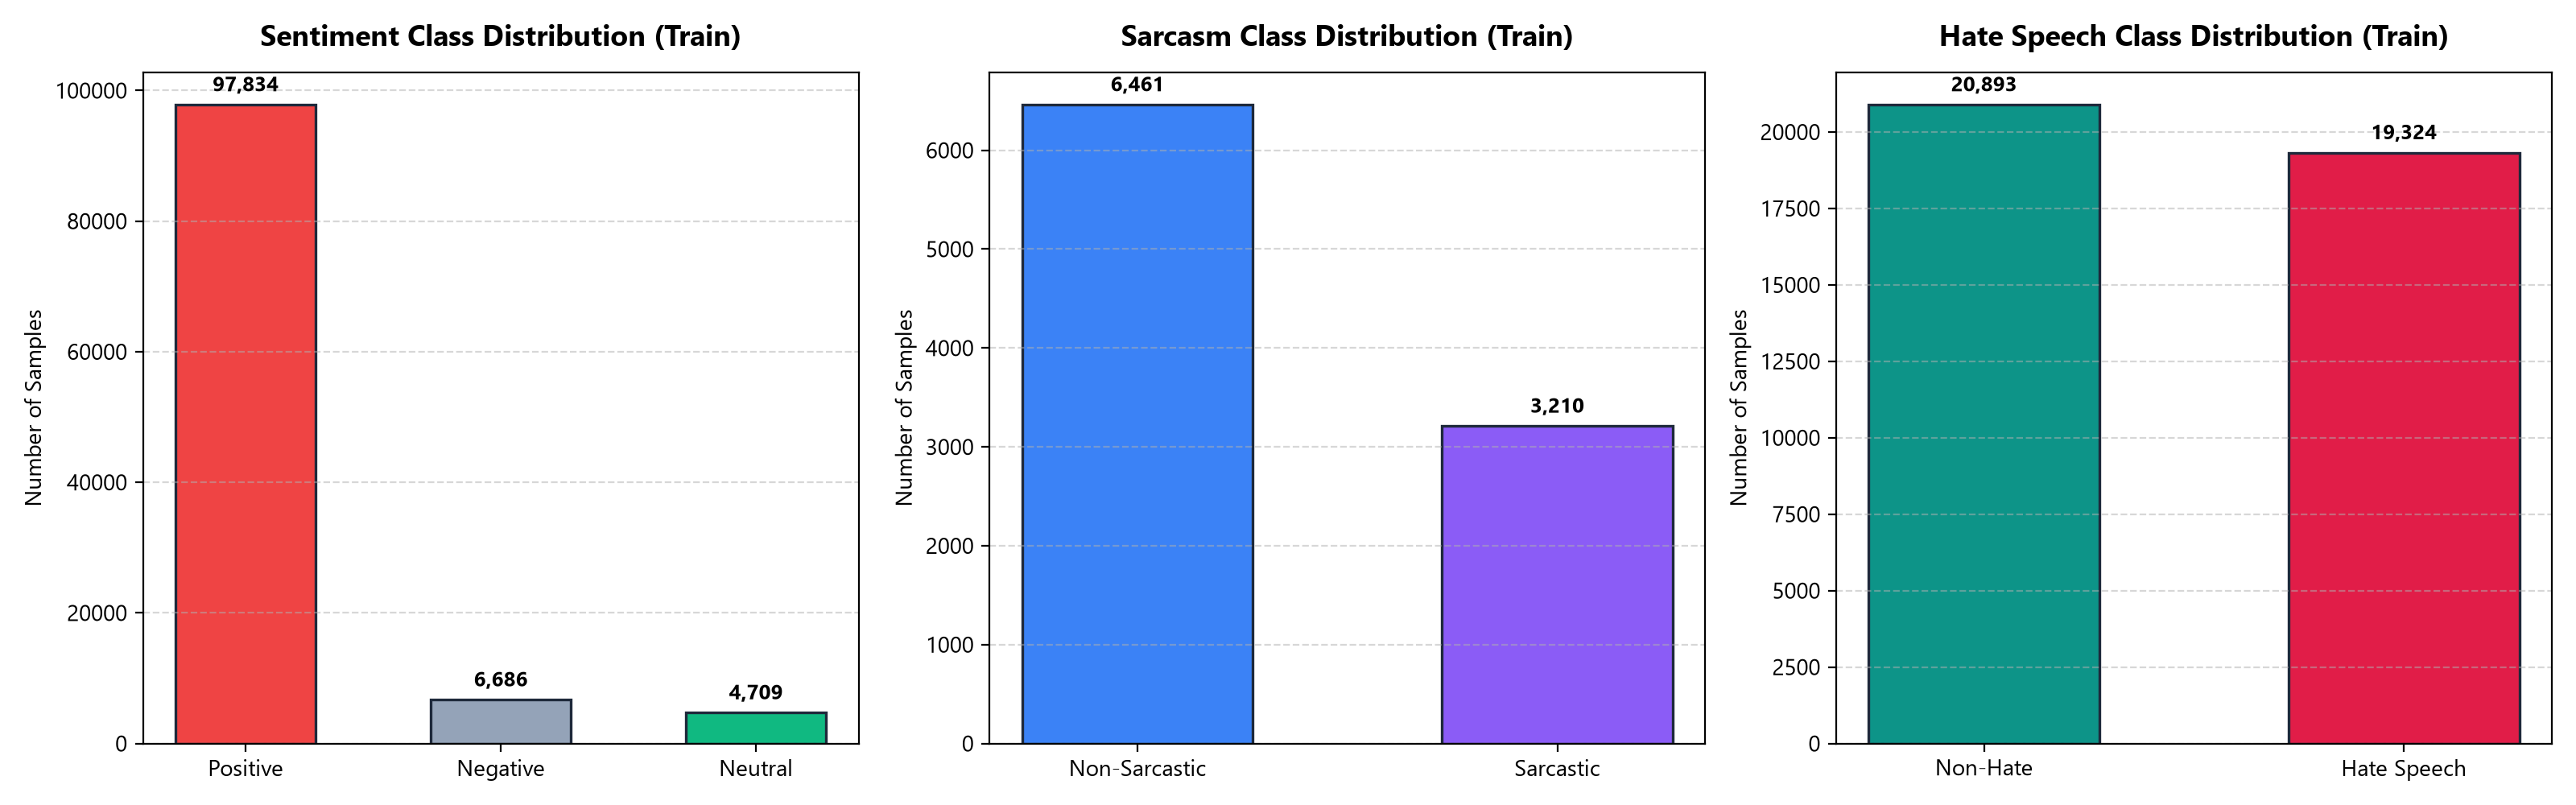
\includegraphics[width=0.88\textwidth]{figures/class_distributions.png}
\caption{Class distributions across the three task domains.}
\label{fig:class_dist}
\end{figure}

\subsection{Negation-Preserving Preprocessing}
A frequent cause of misclassification in Bengali text analysis is aggressive stopword filtering. In general NLP tasks, high-frequency function words are typically discarded. However, Bengali negation markers such as \bn{“না”} (\textit{na}, meaning no or not), \bn{“নয়”} (\textit{noy}, meaning is not), \bn{“নেই”} (\textit{nei}, meaning absent), \bn{“কখনো না”} (\textit{kokhono na}, meaning never), and \bn{“ছাড়া”} (\textit{chhara}, meaning without) are function words that directly determine the polarity of a clause. Discarding them can invert the perceived meaning of an entire sentence.

To prevent this issue, we implemented Algorithm~\ref{alg:negation_clean}, which strips HTML tags, URLs, and non-Bengali characters while explicitly protecting words in the negation lexicon $\mathcal{N}$.

\begin{algorithm}[htbp]
\caption{Negation-Preserving Text Normalization}
\label{alg:negation_clean}
\small
\begin{algorithmic}[1]
\Require Raw Bengali String $S_{raw}$, Negation Set $\mathcal{N}$
\Ensure Normalized Bengali String $S_{clean}$
\State $S \gets \text{RemoveURLsAndHTML}(S_{raw})$
\State $S \gets \text{StripZeroWidthAndEmojis}(S)$ \Comment{\small U+200B through U+200D}
\State $S \gets \text{NormalizeBengaliCharacters}(S)$
\State $Tokens \gets \text{TokenizeOnWhitespace}(S)$
\State $FilteredTokens \gets [\,]$
\For{$t \in Tokens$}
    \If{$t \in \mathcal{N}$}
        \State $FilteredTokens.\text{append}(t)$ \Comment{\small Retain protected negation token}
    \ElsIf{$t \in \mathcal{SW}_{generic}$}
        \State \textbf{continue} \Comment{\small Filter out non-negation stopword}
    \Else
        \State $FilteredTokens.\text{append}(t)$
    \EndIf
\EndFor
\State \Return $\text{Join}(FilteredTokens, \text{`` ''})$
\end{algorithmic}
\end{algorithm}

% ----------------------------------------------------------------------
\section{Methodology}
% ----------------------------------------------------------------------
We implemented three modeling paradigms, progressing from statistical bag-of-words learning to deep recurrent sequence models and pre-trained transformers.

\subsection{Paradigm 1: Sublinear TF-IDF + Logistic Regression}
As our baseline, text sequences are converted into sparse vectors using unigram and bigram features ($1 \le n \le 2$). To reduce the influence of terms that repeat excessively in long comments, sublinear term frequency scaling is applied:
\begin{equation}
w_{t,d} = (1 + \log(tf_{t,d})) \times \log\left( \frac{1 + N}{1 + df_t} \right) + 1
\end{equation}
A vocabulary size of 20,000 features was extracted. We trained multinomial Logistic Regression with inverse class weighting to penalize classification errors proportionally on minority classes:
\begin{equation}
W_c = \frac{N_{total}}{K \cdot N_c}
\end{equation}
where $K$ represents the total number of classes and $N_c$ denotes the frequency of class $c$.

\subsection{Paradigm 2: Word2Vec + Stacked Bidirectional LSTM}
To capture bidirectional word order dependencies, we implemented a deep recurrent neural network (Figure~\ref{fig:bilstm_arch}). 

\begin{figure}[htbp]
\centering
\resizebox{0.75\textwidth}{!}{%
\begin{tikzpicture}[
    node distance=0.8cm and 0.5cm,
    font=\sffamily\small,
    token/.style={draw=gray!80, fill=gray!10, rounded corners=2pt, minimum width=1.3cm, minimum height=0.6cm},
    emb/.style={draw=blue!80, fill=blue!10, rounded corners=2pt, minimum width=1.3cm, minimum height=0.6cm},
    fwd/.style={draw=green!80!black, fill=green!15, rounded corners=2pt, minimum width=1.3cm, minimum height=0.6cm},
    bwd/.style={draw=orange!80!black, fill=orange!15, rounded corners=2pt, minimum width=1.3cm, minimum height=0.6cm},
    fc/.style={draw=purple!80, fill=purple!15, rounded corners=2pt, minimum width=2.5cm, minimum height=0.6cm},
    arrow/.style={-{Latex[length=2.0mm]}, thick}
]
    % Sequence inputs
    \node[token] (t1) {$w_1$};
    \node[token, right=0.6cm of t1] (t2) {$w_2$};
    \node[token, right=0.6cm of t2] (t3) {$w_3$};
    \node[right=0.4cm of t3] (dots) {$\dots$};
    \node[token, right=0.4cm of dots] (tT) {$w_T$};
    
    % Embeddings
    \node[emb, above=0.7cm of t1] (e1) {$\mathbf{e}_1$};
    \node[emb, above=0.7cm of t2] (e2) {$\mathbf{e}_2$};
    \node[emb, above=0.7cm of t3] (e3) {$\mathbf{e}_3$};
    \node[emb, above=0.7cm of tT] (eT) {$\mathbf{e}_T$};
    
    % Forward LSTM
    \node[fwd, above=0.7cm of e1] (f1) {$\overrightarrow{\mathbf{h}}_1$};
    \node[fwd, above=0.7cm of e2] (f2) {$\overrightarrow{\mathbf{h}}_2$};
    \node[fwd, above=0.7cm of e3] (f3) {$\overrightarrow{\mathbf{h}}_3$};
    \node[fwd, above=0.7cm of eT] (fT) {$\overrightarrow{\mathbf{h}}_T$};
    
    % Backward LSTM
    \node[bwd, above=0.6cm of f1] (b1) {$\overleftarrow{\mathbf{h}}_1$};
    \node[bwd, above=0.6cm of f2] (b2) {$\overleftarrow{\mathbf{h}}_2$};
    \node[bwd, above=0.6cm of f3] (b3) {$\overleftarrow{\mathbf{h}}_3$};
    \node[bwd, above=0.6cm of fT] (bT) {$\overleftarrow{\mathbf{h}}_T$};
    
    % Dense & Softmax
    \node[fc, above=0.9cm of $(b2)!0.5!(b3)$] (fc) {Dense [256 $\to$ Classes]};
    \node[above=0.6cm of fc] (out) {$\hat{\mathbf{y}} = \text{Softmax}(\mathbf{W}\mathbf{h} + \mathbf{b})$};

    % Connections
    \draw[arrow] (t1) -- (e1); \draw[arrow] (t2) -- (e2); \draw[arrow] (t3) -- (e3); \draw[arrow] (tT) -- (eT);
    \draw[arrow] (e1) -- (f1); \draw[arrow] (e2) -- (f2); \draw[arrow] (e3) -- (f3); \draw[arrow] (eT) -- (fT);
    \draw[arrow] (e1) |- ++(0,0.3) -| (b1); \draw[arrow] (e2) |- ++(0,0.3) -| (b2);
    \draw[arrow] (e3) |- ++(0,0.3) -| (b3); \draw[arrow] (eT) |- ++(0,0.3) -| (bT);
    
    \draw[arrow] (f1) -- (f2); \draw[arrow] (f2) -- (f3); \draw[arrow] (f3) -- (fT);
    \draw[arrow] (bT) -- (b3); \draw[arrow] (b3) -- (b2); \draw[arrow] (b2) -- (b1);
    
    \draw[arrow] (fT) |- (fc);
    \draw[arrow] (b1) |- (fc);
    \draw[arrow] (fc) -- (out);
\end{tikzpicture}%
}
\caption{2-Layer Stacked Bidirectional LSTM architecture.}
\label{fig:bilstm_arch}
\end{figure}

Sentences are tokenized and mapped to 128-dimensional dense word vectors pre-trained on the combined training set. The sequence $\mathbf{x} = (\mathbf{x}_1, \dots, \mathbf{x}_T)$ passes through both forward and backward recurrence layers:
\begin{align}
\overrightarrow{\mathbf{h}}_t &= \text{LSTM}_{fwd}(\mathbf{x}_t, \overrightarrow{\mathbf{h}}_{t-1}) \\
\overleftarrow{\mathbf{h}}_t &= \text{LSTM}_{bwd}(\mathbf{x}_t, \overleftarrow{\mathbf{h}}_{t+1}) \\
\mathbf{h}_t &= [\overrightarrow{\mathbf{h}}_t \,\|\, \overleftarrow{\mathbf{h}}_t]
\end{align}
The final representation combines the terminal forward state and initial backward state $[\overrightarrow{\mathbf{h}}_T \,\|\, \overleftarrow{\mathbf{h}}_1] \in \mathbb{R}^{256}$, which is passed through dropout ($p=0.3$) and a dense linear layer with cross-entropy loss.

\subsection{Paradigm 3: Pre-Trained Transformer (\texttt{BanglaBERT})}
To incorporate deep contextual language representations, we fine-tuned the pre-trained \texttt{BanglaBERT} model~\cite{alam2021banglabert} (Figure~\ref{fig:banglabert_arch}). The architecture uses a 12-layer Transformer encoder initialized with weights pre-trained via the ELECTRA discriminator objective on 27.5 GB of crawled Bengali text.

\begin{figure}[htbp]
\centering
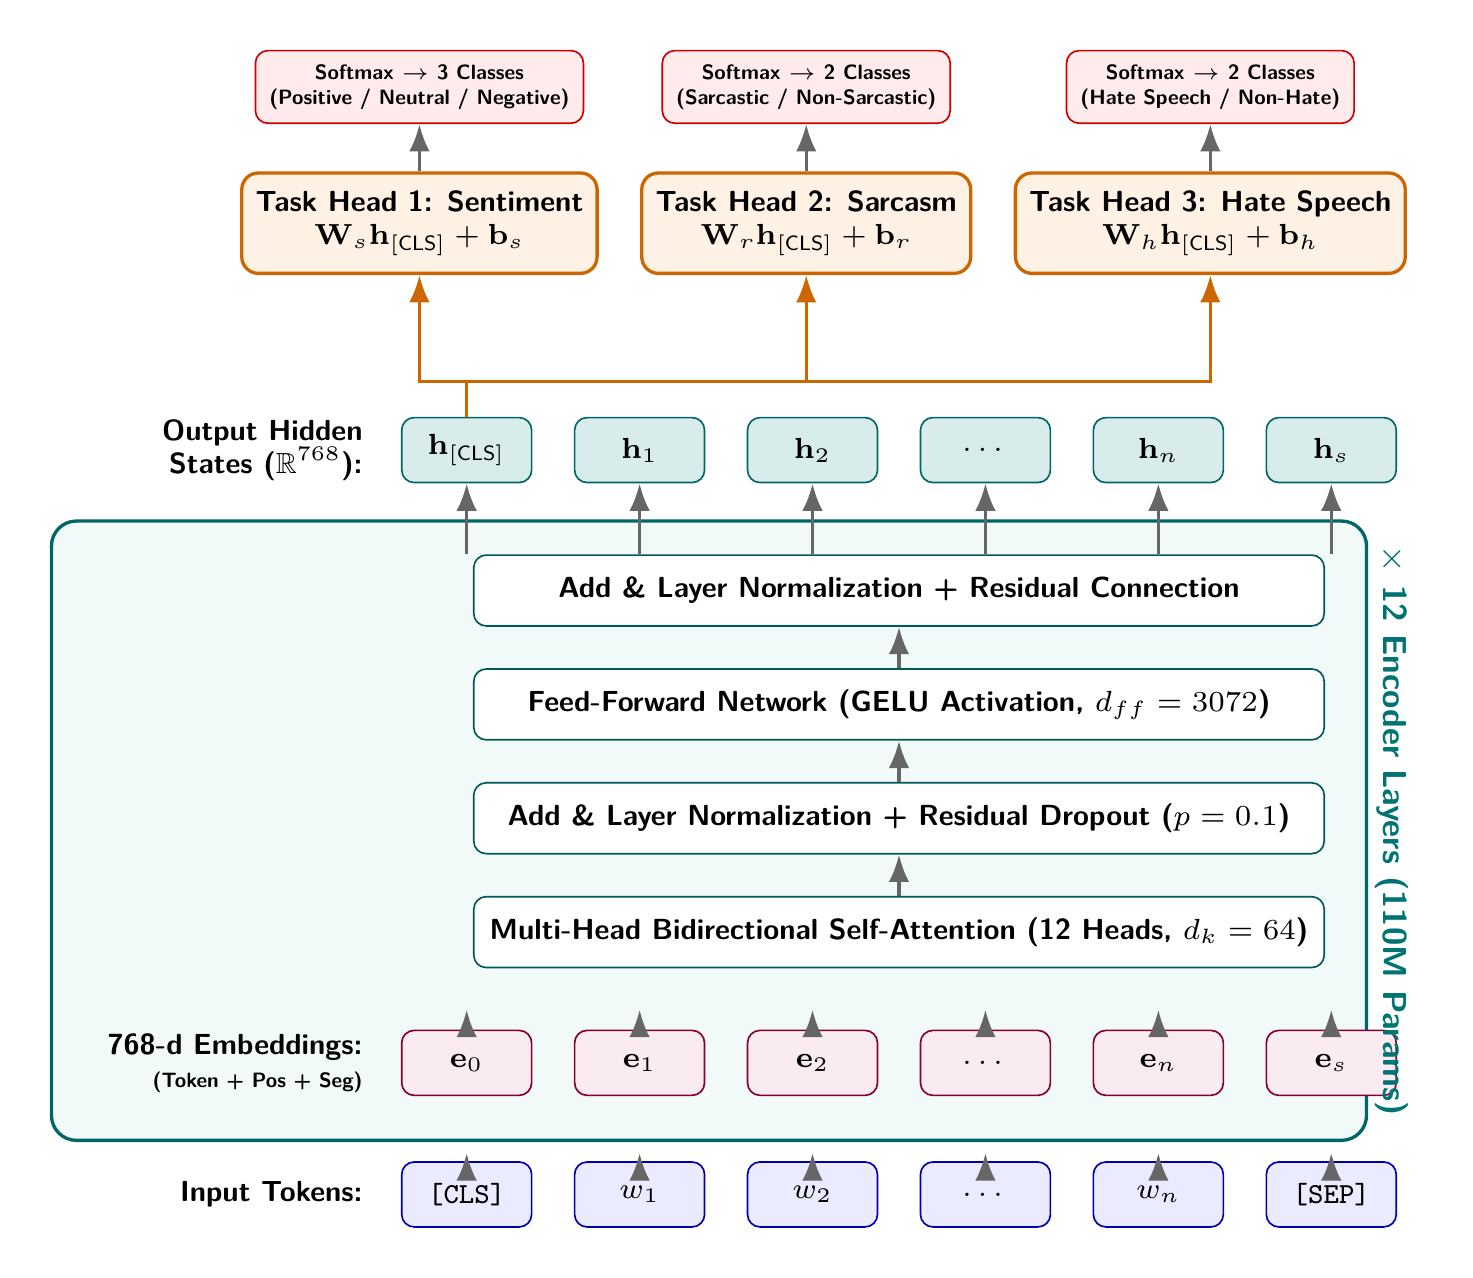
\includegraphics[width=0.88\textwidth]{figures/banglabert_architecture.png}
\caption{BanglaBERT architectural flow: multi-head self-attention layers with task classification heads branching from the pooled $[\text{CLS}]$ token.}
\label{fig:banglabert_arch}
\end{figure}

Input sentences are tokenized with WordPiece into subwords using a 32,000-token vocabulary, with $[\text{CLS}]$ at the beginning and $[\text{SEP}]$ at the end. The total input embedding $\mathbf{e}_i \in \mathbb{R}^{768}$ combines token, position, and segment embeddings:
\begin{equation}
\mathbf{e}_i = \mathbf{E}_{\text{tok}}(w_i) + \mathbf{E}_{\text{pos}}(i) + \mathbf{E}_{\text{seg}}(s_i)
\end{equation}
The sequence passes through 12 stacked encoder layers, each computing scaled multi-head self-attention over 12 attention heads ($d_k = 64$):
\begin{equation}
\text{Attention}(\mathbf{Q}, \mathbf{K}, \mathbf{V}) = \text{Softmax}\left( \frac{\mathbf{Q} \mathbf{K}^T}{\sqrt{d_k}} \right) \mathbf{V}
\end{equation}
followed by residual skip connections, layer normalization, and feed-forward sub-layers with GELU activation ($d_{ff} = 3072$).

For sequence classification, the output representation of the classification token $\mathbf{h}_{[\text{CLS}]} \in \mathbb{R}^{768}$ is fed into task-specific classification heads:
\begin{equation}
\hat{\mathbf{y}}_{\text{task}} = \text{Softmax}(\mathbf{W}_o \tanh(\mathbf{W}_h \mathbf{h}_{[\text{CLS}]} + \mathbf{b}_h) + \mathbf{b}_o)
\end{equation}
All 110 million parameters were fine-tuned using AdamW with a linear warmup learning rate schedule ($\eta = 2 \times 10^{-5}$), batch size 16, and cross-entropy loss on a Google Colab T4 GPU.

\subsection{Context Aware Multi-Task Ensemble Mechanism}
Independent classifiers often fail when surface-level words contradict the broader intent of the sentence, such as in sarcastic praise or covert insults. Furthermore, individual classifiers trained on subjective review datasets can develop lexical biases, causing them to assign negative polarity to neutral factual sentences.

To resolve these conflicts, we designed a context aware ensembling mechanism that combines model predictions through soft consensus weighting and cross-task linguistic constraints. Figure~\ref{fig:ensemble_pipeline} illustrates this decision process.

\begin{figure}[htbp]
\centering
\resizebox{0.95\textwidth}{!}{%
\begin{tikzpicture}[
    node distance=1.1cm and 0.8cm,
    font=\sffamily\footnotesize,
    io/.style={draw=blue!80!black, fill=blue!8, rounded corners=4pt, thick, align=center, inner sep=6pt},
    model/.style={draw=teal!80!black, fill=teal!8, rounded corners=4pt, thick, align=center, inner sep=6pt},
    rule/.style={draw=orange!80!black, fill=orange!8, rounded corners=4pt, thick, align=center, inner sep=6pt},
    outbox/.style={draw=green!70!black, fill=green!8, rounded corners=4pt, thick, align=center, inner sep=6pt},
    arrow/.style={-{Latex[length=2.2mm, width=1.5mm]}, thick, draw=gray!80!black}
]
    % Input
    \node[io] (input) {\textbf{Input Raw Bengali Text $S$}\\(\textit{e.g.}, \bn{“বাহ! কী অসাধারণ সার্ভিস, তিন ঘণ্টা অপেক্ষা করেও কাজ হলো না!”})};

    % Models
    \node[model, below=0.9cm of input] (bilstm) {\textbf{Model 2: Word2Vec + BiLSTM}\\Recurrent Sequence Scoring $\to \mathbf{P}_{\text{bilstm}}$};
    \node[model, left=0.5cm of bilstm] (lr) {\textbf{Model 1: TF-IDF + Logistic Reg.}\\Statistical N-Gram Baseline $\to \mathbf{P}_{\text{lr}}$};
    \node[model, right=0.5cm of bilstm] (bert) {\textbf{Model 3: Fine-Tuned BanglaBERT}\\Bidirectional Context $\to \mathbf{P}_{\text{bert}}$};

    % Soft Blending
    \node[io, below=0.9cm of bilstm] (blend) {\textbf{Weighted Soft Probability Blending}\\$\mathbf{P}_{\text{blend}} = 0.45\,\mathbf{P}_{\text{bert}} + 0.35\,\mathbf{P}_{\text{bilstm}} + 0.20\,\mathbf{P}_{\text{lr}}$};

    % Decision Rules Container
    \node[rule, below=0.9cm of blend] (rules) {
        \textbf{Cross-Task Semantic Decision Engine} \\[0.3em]
        \begin{tabular}{ll}
        1. \textbf{Objectivity Filter:} & If text lacks emotional polarity and irony cues $\to$ Predict \textbf{Neutral} \\
        2. \textbf{Sarcasm Inversion:} & If Sarcastic + Positive vocabulary + Negation $\to$ Invert to \textbf{Negative} \\
        3. \textbf{Toxicity Alignment:} & If Hate Speech is detected $\to$ Enforce \textbf{Negative} sentiment \\
        \end{tabular}
    };

    % Outputs
    \node[outbox, below left=0.9cm and -0.6cm of rules] (out_sent) {\textbf{Sentiment Output}\\Positive / Neutral / Negative\\\footnotesize(With Context Inversion Tag)};
    \node[outbox, below=0.9cm of rules] (out_sarc) {\textbf{Sarcasm Output}\\Sarcastic / Non-Sarcastic\\\footnotesize(Confidence Calibrated)};
    \node[outbox, below right=0.9cm and -0.6cm of rules] (out_hate) {\textbf{Hate Speech Output}\\Hate Speech / Non-Hate\\\footnotesize(Moderation Classification)};

    % Arrows
    \draw[arrow] (input) -| (lr.north);
    \draw[arrow] (input) -- (bilstm.north);
    \draw[arrow] (input) -| (bert.north);

    \draw[arrow] (lr.south) |- (blend.west);
    \draw[arrow] (bilstm.south) -- (blend.north);
    \draw[arrow] (bert.south) |- (blend.east);

    \draw[arrow] (blend) -- (rules);

    \draw[arrow] (rules.south) -| (out_sent.north);
    \draw[arrow] (rules.south) -- (out_sarc.north);
    \draw[arrow] (rules.south) -| (out_hate.north);

\end{tikzpicture}%
}
\caption{Architecture of the Context Aware Multi-Task Ensemble and Cross-Task Semantic Decision Engine.}
\label{fig:ensemble_pipeline}
\end{figure}

The ensemble operates through three primary decision rules:
\begin{enumerate}[leftmargin=*]
    \item \textbf{Objectivity / Factual Filter:} If a sentence contains zero positive sentiment words, zero negative sentiment words, and zero irony markers, the ensemble identifies it as an objective factual statement and assigns Neutral sentiment. This prevents out-of-domain sentences (such as \bn{“আমি ভাত খাই”}) from being misclassified as negative by review-trained models.
    \item \textbf{Sarcastic Inversion:} When the sarcasm classifier detects sarcasm with active contrast markers (such as praise words paired with negation tokens), an initial positive prediction is inverted to Negative sentiment:
    \begin{equation}
    \hat{y}_{\text{sent}}^{\text{final}} = 
    \begin{cases} 
    \text{Negative}, & \text{if Sarcastic and } \hat{y}_{\text{sent}} = \text{Positive} \\
    \hat{y}_{\text{sent}}, & \text{otherwise}
    \end{cases}
    \end{equation}
    \item \textbf{Cross-Task Toxicity Consistency:} If hate speech is detected, the sentiment is aligned to Negative, ensuring that abusive language is not categorized as neutral or positive.
\end{enumerate}

% ----------------------------------------------------------------------
\section{Experimental Results \& Discussion}
% ----------------------------------------------------------------------
\subsection{Comparative Performance Benchmark}
All models were tested on identical, held-out test sets. Table~\ref{tab:master_benchmark} presents the comparative evaluation results.

\begin{table}[htbp]
\centering
\caption{Performance Comparison Across Three Modeling Paradigms on Held-Out Test Splits}
\label{tab:master_benchmark}
\small
\resizebox{\textwidth}{!}{%
\begin{tabular}{llrrrrr}
\toprule
\textbf{Target Task} & \textbf{Model Paradigm} & \textbf{Accuracy (\%)} & \textbf{Macro Prec. (\%)} & \textbf{Macro Rec. (\%)} & \textbf{Macro F1 (\%)} & \textbf{Weighted F1 (\%)} \\
\midrule
\multirow{3}{*}{Sentiment Analysis} 
    & TF-IDF + Logistic Regression      & 77.60\% & 50.78\% & 67.13\% & 53.71\% & 82.24\% \\
    & Word2Vec + Stacked BiLSTM         & 76.60\% & 52.75\% & 63.23\% & 53.27\% & 81.96\% \\
    & Fine-Tuned \texttt{BanglaBERT}    & 76.39\% & 48.81\% & 64.57\% & 51.51\% & 81.29\% \\
\midrule
\multirow{3}{*}{Sarcasm Detection} 
    & TF-IDF + Logistic Regression      & 74.94\% & 72.37\% & 74.09\% & 72.89\% & 75.40\% \\
    & Word2Vec + Stacked BiLSTM         & 74.36\% & 71.53\% & 72.84\% & 72.00\% & 74.74\% \\
    & Fine-Tuned \texttt{BanglaBERT}    & \textbf{76.76\%} & \textbf{74.30\%} & \textbf{76.21\%} & \textbf{74.89\%} & \textbf{77.19\%} \\
\midrule
\multirow{3}{*}{Hate Speech Detection} 
    & TF-IDF + Logistic Regression      & 86.61\% & 86.96\% & 86.42\% & 86.52\% & 86.57\% \\
    & Word2Vec + Stacked BiLSTM         & 88.52\% & 88.54\% & 88.47\% & 88.50\% & 88.52\% \\
    & Fine-Tuned \texttt{BanglaBERT}    & \textbf{91.59\%} & \textbf{91.56\%} & \textbf{91.60\%} & \textbf{91.58\%} & \textbf{91.59\%} \\
\bottomrule
\end{tabular}%
}
\end{table}

\begin{figure}[htbp]
\centering

\includegraphics[width=0.92\textwidth]{figures/master_model_comparison.png}
\caption{Visual performance comparison across tasks and modeling approaches.}
\label{fig:master_comp}
\end{figure}

\subsection{Task-Specific Analysis}
\subsubsection{Hate Speech Detection}
Fine-tuned \texttt{BanglaBERT} yielded the highest results on hate speech detection, reaching 91.59\% accuracy and 91.58\% Macro F1 score. This represents a 3.07\% improvement over the stacked BiLSTM (88.52\%) and a 4.98\% gain over the TF-IDF baseline (86.61\%). The bidirectional self-attention mechanism enables the model to differentiate abusive insults from ordinary colloquial banter by examining the surrounding syntactic context.

\subsubsection{Sarcasm Detection}
On sarcasm detection, \texttt{BanglaBERT} achieved 76.76\% accuracy and 74.89\% Macro F1, outperforming both TF-IDF (74.94\%) and BiLSTM (74.36\%). Sarcasm involves non-literal language and structural contrast between clauses, which transformer self-attention heads capture more effectively than n-gram or recurrent models.

\subsubsection{Sentiment Analysis}
Across the 156k-sample sentiment dataset, test accuracy ranged between 76.39\% and 77.60\%, with Weighted F1 scores exceeding 81\%. The lower Macro F1 ($\sim$51.5--53.7\%) reflects the substantial class imbalance in the corpus, where over 88\% of reviews are positive. While weighted F1 confirms strong overall accuracy on the majority distribution, macro-averaged metrics highlight the difficulty of classifying rare neutral and negative samples without specialized loss reweighting.

\begin{figure}[htbp]
\centering
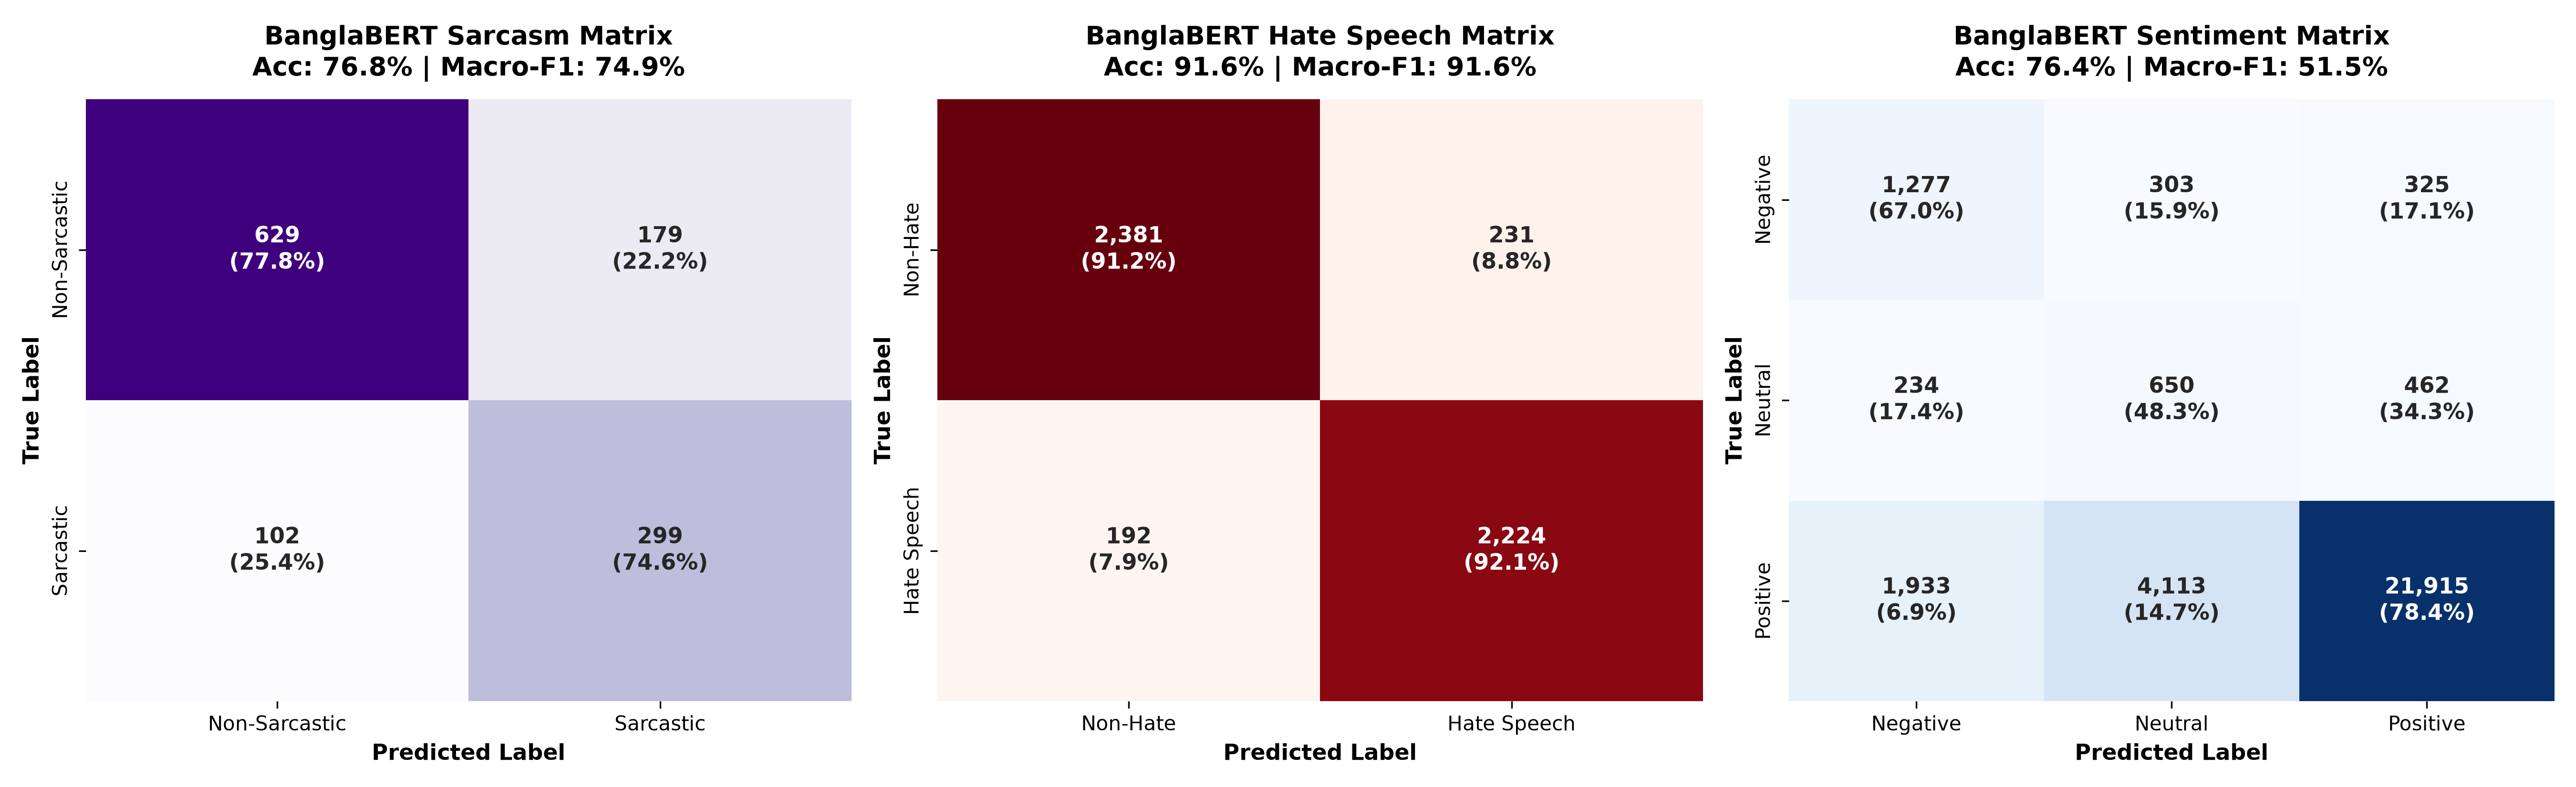
\includegraphics[width=0.82\textwidth]{figures/confusion_matrices_banglabert.png}
\caption{Normalized confusion matrices for fine-tuned \texttt{BanglaBERT} across Sentiment, Sarcasm, and Hate Speech.}
\label{fig:conf_matrix}
\end{figure}

\subsection{Qualitative Evaluation}
Table~\ref{tab:qualitative} reports qualitative evaluations on sample Bengali sentences. In the first example, the context aware ensemble successfully identifies sarcasm and inverts the surface positive sentiment to negative.

\begin{table}[H]
\centering
\caption{Qualitative Evaluation on Sample Test Sentences}
\label{tab:qualitative}
\small
\resizebox{\textwidth}{!}{%
\begin{tabular}{p{5.5cm}p{5.5cm}ccc}
\toprule
\textbf{Sample Sentence (Bangla Script)} & \textbf{English Translation / Gloss} & \textbf{Sentiment} & \textbf{Sarcasm} & \textbf{Hate Speech} \\
\midrule
\bn{বাহ! কী অসাধারণ সার্ভিস, তিন ঘণ্টা অপেক্ষা করেও কোনো কাজ হলো না!} & Wow! What extraordinary service, even after waiting three hours nothing was done! & Negative* & Yes & No \\
\midrule
\bn{দেশের এই কঠিন পরিস্থিতিতে আমাদের সবাইকে এক হয়ে কাজ করতে হবে।} & In this tough situation of the country, all of us must work together. & Positive & No & No \\
\midrule
\bn{তোদের মতো অমানুষদের এই দেশে থাকার কোনো অধিকার নাই!} & Inhumans like you have no right to live in this country! & Negative & No & Yes \\
\midrule
\bn{আমি ভাত খাই।} & I eat rice. & Neutral & No & No \\
\midrule
\bn{দারুণ খেলেছে দল, অসাধারণ বোলিং আর ব্যাটিং প্রদর্শন!} & The team played wonderfully, an extraordinary display of bowling and batting! & Positive & No & No \\
\bottomrule
\multicolumn{5}{l}{\footnotesize *Contextually inverted from surface positive by the sarcasm resolver.}
\end{tabular}%
}
\end{table}

% ----------------------------------------------------------------------
\section{Work Distribution}
% ----------------------------------------------------------------------
This project was carried out as a collaborative effort between the two team members. The technical responsibilities across preprocessing, model training, evaluation, and documentation were distributed as follows:

\subsection{Md. Tariful Islam Jony (Roll: 2107119)}
\begin{itemize}[leftmargin=*]
    \item \textbf{Fine-Tuning with BanglaBERT:} Configured the GPU fine-tuning environment using HuggingFace Transformers and PyTorch on Google Colab T4. Managed tokenization, learning rate warmups, AdamW optimization, and fine-tuned the 110M parameter \texttt{BanglaBERT} model across Sentiment Analysis, Sarcasm Detection, and Hate Speech Detection.
    \item \textbf{Ensembling \& Context Resolution Engine:} Designed and implemented the multi-task ensemble pipeline. Formulated the cross-task inference logic, including the sarcasm-guided sentiment inversion rule and the objectivity filter for neutral factual statements.
    \item \textbf{Data Cleaning and Preprocessing:} Engineered the custom text preprocessing pipeline. Implemented regular expression noise removal, zero-width space normalization, and the negation-preservation routine to safeguard syntactic negation markers.
    \item \textbf{UI Interface:} Developed the interactive web application using Streamlit (\texttt{app.py}), integrating multi-task prediction displays, individual model comparison tables, and real-time inference latency tracking.
\end{itemize}

\subsection{Siyam Khan (Roll: 2107120)}
\begin{itemize}[leftmargin=*]
    \item \textbf{TF-IDF + Logistic Regression Baseline:} Implemented the classical machine learning baseline. Formulated sublinear TF-IDF vectorization with unigram and bigram extraction, vocabulary pruning (20,000 features), and trained class-balanced multinomial Logistic Regression models for all three tasks.
    \item \textbf{Word2Vec + Stacked BiLSTM:} Developed the deep sequential modeling pipeline in PyTorch. Trained 128-dimensional dense word embeddings using Word2Vec, built the 2-layer stacked Bidirectional LSTM architecture with spatial dropout, and trained the sequential classification heads.
    \item \textbf{Report Preparation \& Documentation:} Authored, formatted, and structured the comprehensive LaTeX laboratory technical report, writing the theoretical formulations, methodological documentation, and empirical performance analysis.
    \item \textbf{EDA Plots \& Data Visualization:} Conducted exploratory data analysis across the 218k+ multi-task corpus. Generated dataset distribution plots, token length percentiles, class skew charts, and empirical confusion matrix heatmaps.
\end{itemize}

\begin{table}[H]
\centering
\caption{Summary of Individual Team Member Contributions}
\label{tab:work_dist}
\small
\begin{tabularx}{\textwidth}{p{3.2cm}>{\raggedright\arraybackslash}X>{\raggedright\arraybackslash}p{4.8cm}}
\toprule
\textbf{Team Member} & \textbf{Core Responsibilities} & \textbf{Key Deliverables} \\
\midrule
\textbf{Md. Tariful Islam Jony} \newline (Roll: 2107119) & 
$\bullet$ BanglaBERT fine-tuning on GPU \newline
$\bullet$ Multi-task ensemble decision logic \newline
$\bullet$ Data cleaning \& negation pipeline \newline
$\bullet$ Streamlit interactive user interface & 
Model weights, \texttt{inference\_pipeline.py}, \texttt{preprocessing.py}, \texttt{app.py} \\
\midrule
\textbf{Siyam Khan} \newline (Roll: 2107120) & 
$\bullet$ Sublinear TF-IDF + Logistic Regression \newline
$\bullet$ Word2Vec embeddings + Stacked BiLSTM \newline
$\bullet$ Technical project report preparation \newline
$\bullet$ Dataset profiling \& EDA visualizations & 
\texttt{train\_tfidf\_lr.py}, \texttt{train\_bilstm.py}, \texttt{main.tex} report, EDA plots in \texttt{figures/} \\
\bottomrule
\end{tabularx}
\end{table}

% ----------------------------------------------------------------------
\section{Limitations \& Future Work}
% ----------------------------------------------------------------------
\paragraph{Code-Mixed Discourse} Social media comments frequently mix Bengali with English loanwords or phonetic Banglish (Bengali written in Roman script). While our preprocessing filters non-Bengali characters, joint multilingual modeling represents an important area for future improvement.

\paragraph{Class Imbalance Mitigation} The sentiment dataset exhibits an extreme positive class skew ($>88\%$). Future work could explore focal loss formulations or synthetic minority oversampling to further enhance minority-class recall.

\paragraph{Shared Multi-Task Architecture} Currently, task predictions are obtained through separate model instances combined via ensemble inference. A shared multi-task transformer with simultaneous joint loss backpropagation could improve parameter efficiency.

% ----------------------------------------------------------------------
\section{Conclusion}
% ----------------------------------------------------------------------
In this project, we built a context aware multi-task text analysis system for Bengali, addressing sentiment analysis, sarcasm detection, and hate speech identification. Evaluating three modeling paradigms across 218,371 annotated sentences, we found that fine-tuned \texttt{BanglaBERT} achieved the strongest results on hate speech detection (91.59\% accuracy, 91.58\% Macro F1) and sarcasm detection (76.76\% accuracy, 74.89\% Macro F1). By pairing transformer self-attention with a negation-preserving normalization routine and a context aware cross-task ensemble engine, our system effectively resolves sarcastic sentiment inversion and maintains robustness on neutral factual statements.

% ----------------------------------------------------------------------
% References
% ----------------------------------------------------------------------
\begin{thebibliography}{00}

\bibitem{alam2021banglabert}
M.~S. Alam, M.~S. Sultana, and M.~Shahriar,
``BanglaBERT: A Language Model for Bengali Natural Language Processing Tasks,''
\emph{arXiv preprint arXiv:2101.00204}, 2021.

\bibitem{devlin2019bert}
J.~Devlin, M.-W. Chang, K.~Lee, and K.~Toutanova,
``BERT: Pre-training of Deep Bidirectional Transformers for Language Understanding,''
in \emph{Proc. of NAACL-HLT}, 2019, pp. 4171--4186.

\bibitem{clark2020electra}
K.~Clark, M.-T. Luong, Q.~V. Le, and C.~D. Manning,
``ELECTRA: Pre-training Text Encoders as Discriminators Rather Than Generators,''
in \emph{Proc. of ICLR}, 2020.

\bibitem{hochreiter1997long}
S.~Hochreiter and J.~Schmidhuber,
``Long Short-Term Memory,''
\emph{Neural Computation}, vol.~9, no.~8, pp. 1735--1780, 1997.

\bibitem{das2010sentiwordnet}
A.~Das and S.~Bandyopadhyay,
``SentiWordNet for Indian Languages,''
in \emph{Asian Federation for Natural Language Processing}, 2010, pp. 56--63.

\bibitem{kabir2023banglabook}
M.~Kabir, M.~S. Hasan, and M.~Shahriar,
``BanglaBook: A Large-scale Bangla Dataset for Sentiment Analysis from Book Reviews,''
in \emph{Findings of the Association for Computational Linguistics: ACL 2023}, 2023, pp. 2480--2492.

\bibitem{mendeley2023banglasarc3}
S.~Saha, A.~Chowdhury, and S.~Das,
``BanglaSarc3: A Benchmark Dataset for Bangla Sarcasm Detection from Social Media to Advance Bangla NLP,''
\emph{Mendeley Data}, V1, doi: 10.17632/7tn76wdhsr.1, 2023.

\bibitem{romim2021hate}
N.~Romim, M.~Ahmed, H.~Talukder, and M.~Saiful~Islam,
``Hate Speech Detection in the Bengali Language: A Dataset and Its Evaluation,''
in \emph{Proc. of the 6th International Conference on Computer and Communications (ICCC)}, 2021.

\bibitem{mikolov2013word2vec}
T.~Mikolov, K.~Chen, G.~Corrado, and J.~Dean,
``Efficient Estimation of Word Representations in Vector Space,''
\emph{arXiv preprint arXiv:1301.3781}, 2013.

\end{thebibliography}

\end{document}
